\section{Frontenddesign \textnormal{\textsf{\small{Niklas Schuster}}}}
\subsection{Framework \& Assets}
Das Design des Frontends basiert auf dem Open-Source Framework Bootstrap. Das von Twitter entwickelte Framework enthält HTML, CSS und JavaScript Elemente für die Entwicklung moderner Responsive Web Applikationen und umfasst Styles für Formulare, Tabellen, Buttons, Typographie, Navigation und ähnliches. Die Basis des Frameworks bildet das 12er Grid System, welches über verschiedeneGeräte- oder Viewport-Größen skaliert und damit Build-In Full Responsive Webdesign unterstützt. Dabei werden Elemente in Zeilen und  Spalten angeordnen. Eine Beispielanordnung zeigt Abbildung \ref{Grid}. Des weiteren wird für die Typografie das das Iconic Font und CSS Toolkit "Font Awsome 4.7" verwendet, welches über CDN wie folgt eingebunden wird: \\ \verb!<script src="https://use.fontawesome.com/8573f20f3e.js"></script>!\\
Das einbinden von Bootstrap geschieht ebenfalls über CDN. Der Code ist zu findem im \verb!<head></head>! Tag der Seiten \textit{index.html} sowie \textit{home.html} (vollständiger Code liegt im Anhang bei). Darüber hinaus benötigen einige Bootstrap Funktionen die JavaScript Bibliothek JQuery und Ajax, welches zur asynchronen Datenübertragung zwische Browser und Server genutzt wird. Als grafische Vorlage für das Interface dient in Abbildung \ref{fig:Color} dargestelltes Farbschema. Dabei bilden die Schwarzstufen die Grundfarben und die Orangtöne werden als Akzentfarbe für Buttons genutzt.

\begin{figure}
	\centering
	
\includegraphics[scale=0.32]{img/Capture.PNG}
	\captionsetup{format=hang}
	\caption[Farbschema]{\label{fig:Color}Farbschema}
\end{figure}
\begin{figure}
	\centering
	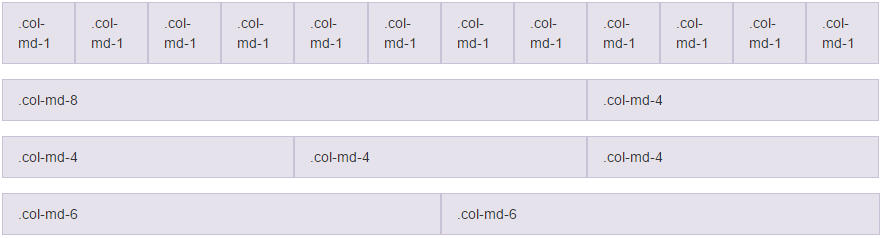
\includegraphics[scale=0.7]{img/Capture2.PNG}
	\captionsetup{format=hang}
	\caption[Beispiel Bootstrap Grid]{\label{fig:Grid}Beispiel Bootstrap Grid \cite{B}}

	\begin{lstlisting}[caption={Code für Abbuildung \ref{fig:Grid} \cite{B}}, label={lst:Database Query Core Node}]
<div class="row">
  <div class="col-md-1">.col-md-1</div>
  <div class="col-md-1">.col-md-1</div>
  <div class="col-md-1">.col-md-1</div>
  <div class="col-md-1">.col-md-1</div>
  <div class="col-md-1">.col-md-1</div>
  <div class="col-md-1">.col-md-1</div>
  <div class="col-md-1">.col-md-1</div>
  <div class="col-md-1">.col-md-1</div>
  <div class="col-md-1">.col-md-1</div>
  <div class="col-md-1">.col-md-1</div>
  <div class="col-md-1">.col-md-1</div>
  <div class="col-md-1">.col-md-1</div>
</div>
<div class="row">
  <div class="col-md-8">.col-md-8</div>
  <div class="col-md-4">.col-md-4</div>
</div>
<div class="row">
  <div class="col-md-4">.col-md-4</div>
  <div class="col-md-4">.col-md-4</div>
  <div class="col-md-4">.col-md-4</div>
</div>
<div class="row">
  <div class="col-md-6">.col-md-6</div>
  <div class="col-md-6">.col-md-6</div>
</div>
\end{lstlisting}
\end{figure}

\subsection{Landingpage (index.html)}

Die Landigpage \textit{index.html} beinhaltet größtenteils das Registrierungs- und Anmeldeformular. Die Login sowie die Registrierung sind beide durch einen Button erreichbar der ein Standard Bootstrap Modal öffnet. Dieses ist durch zwei Tabs geteilt in den Login und die Registrierun. Für die Registrierung wird lediglich der Name des zu führenden Unternehmens benötigt sowie ein Password. Mit diesen Daten erfolgt auch der Anmeldeprozess, hierbei hat der Spieler die Möglichkeit durch das aktivieren einer Checkbox sich dauerhaft auf dem Server anzumelden. Neben dem Login/Registrierungsbutton der ebenso wie unser EARTHBOUND Logo auf der Seite zentriert angezeigt wird, beinhaltet die Landingpage noch eine Navbar. Diese ist am oberen Rand fixiert und transparent, ebenso wie die Buttons die sich darauf befinden. Es gibt drei links ausgerichtete Buttons für das Impressum, die Datenschutzerklärung und eine FAQ, welche auch als Art Spielanleitung angesehen werden kann. Des weiteren sind zwei rechts ausgerichtete Buttons in der Navbar. Diese sind dazu dar die Spieler anzuzeigen, welche gerade aktiv das Spiel spielen, sowie eine Highscore Liste darzustellen, welche die besten Spieler anzeigt die das Spiel bereits abgeschlossen haben. Auch die Buttons in der Navbar öffnen Modals in dem der Content angezeigt wird. Die FAQ sind speziell als Panele in einem Bootstrap-Accordion eingebunden um die Fragen möglichst übersichtlich zu halten.
Ansonsten ist die Seite im Hintergrund mit einem Video mit transparenten schwarzen Overlay versehen, welches als MP4 und WebM eingebunden ist, somit sollte das Video von jedem Browser unterstützt werden.
\begin{figure}
	\centering
	
\includegraphics[scale=0.3]{img/mock.png}
	\captionsetup{format=hang}
	\caption[Landingpage Mockup]{\label{fig:landingpage}Landingpage Mockup}
\end{figure}
\subsection{Dashboard (home.html)}
Die Seite \textit{home.html} ist die Hauptseite des Spiels, auf welcher der Spieler dauerhaft verbleibt und entsprechende Subseiten dynamisch auf die Seite geladen werden, ohne das die Seite neu geladen wird. Aufgrund dessen ist die Seite in bestimmte Bereiche unterteilt. Am linken Rand befindet sich die Sidebar mit dazugehörigen Verweisen. Es gibt jeweils Subseiten für: Dashboard, Marketing, Human Resources, Produktion, Sales, Accounts, Research und Finances. Die Sidebar ist mit einem Hintergrundbild und einem transparenten schwarzen Overlay versehen, wie auch das Video auf der Landingpage. Der aktive Link in der Sidebar wird jeweils weiß hinterlegt und mit einem kleinen Dreieck versehen. An die Sidebar anschließend ist der Header der Seite mit Navbar. Die Navbar ist am oberen Rand fixiert und beinhaltet links ausgerichtet den Namen des Unternehmens und das aktuelle Datum, sowie rechts ausgerichtet Statusanzeigen für das Sichtguthaben, die momentane Lagerauslastung und die Anzahl an Mitarbeitern die derzeit im Unternehmen beschäftigt sind. Daneben gibt es noch einen Button dem es dem Spieler ermöglicht sich vom Server abzumelden. Den Rest der Seite nimmt ein \verb!<div>! Container mit der ID \textit{content} ein. In diesen wird der Inhalt der Unterseiten geladen, welche in den nächsten Abschnitten beschrieben werden.

\subsubsection{Dasboard}
 Die erste Unterseite ist das eigentliche Dashboard des Spiels. Hier erhält der Spieler in Form von Diagrammen einen Überblick über die Lage seines Unternehmens. Dafür wird die JavaScript Bibliothek Chart.js benutzt\cite{C}. Die Bibliothek wird benutzt um Diagramme auf Basis von HTML5, CSS3 und JavaScript generieren zu können. Der Inhalt der Seite ist durch zwei Cards in zwei Hälften geteilt. Auf der linken Seite befindet sich ein Radar Chart, welches dem Spieler Informationen zu seinen aktuellen Kennzahlen zeigt, sowie die Werte der Kennzahlen aus der letzten Periode, damit der Spieler möglichst leicht die Entwicklung seines Unternehmens verfolgen kann. Auf der rechten Seite sieht der Spieler ein Bar Chart, welches für jedes abgeschlossene Jahr Aufwendungen und Erträge des Unternehmens gegenüberstellt und einen Eindruck über die Wirtschaftlichkeit des Unternehmens gibt. Des weiteren wird der Marktanteil des Unternehmens in Relation zu allen anderen Unternehmen amMarkt angezeigt, dafür wird ein Polar Area Chart verwendet.

 \subsubsection{Marketing}
 Auf der Marketingseite wird dem Spieler die Möglichkeit gegeben Marketingkampagnen für sein unternehmen zu starten. Diese Seite, wie auch alle nachfolgenden, verwendet nur eine \textit{card}. Diese ist mit dem Grid-System in zwei gleich große Spalten aufgeteilt, wobei die linke Spalte wiederum in zwei gleich große Spalten aufgeteilt ist. In der linken beiden Spalten befinden sich jeweils zwei Panele untereinander worin dem Spieler Information über alle möglichen Kapagnen gegeben wird, wie z.B. die anfallenden kosten pro Tag und die benötigte Anzahl an Mitarbeitern. Die rechte Spalte wird dazu genutzt alle aktiven Kampagnen anzuzeigen. Dafür wird ein \textit{Panel} genutzt in das für jede Kampagne ein \textit{list-group-item} einer \textit{list-group} erstellt wird. Dort ist die Art der Kampagne sowie die Gesamtkosten aufgelistet. Außerdem gibt es für jeden Eintrag ein \textit{badge} welches die noch verbleibende Laufzeit anzeigt. Zum erstellen neuer Kampagnen befindet sich ein Button in der rechten oberen Ecke der \textit{card}. Dieser öffnet ein \textit{Modal} in dem per \textit{dropdown} die Art der Kampagne ausgewählt werden kann und über ein Input Feld die Dauer den gewünschten Kampagen angegeben werden kann.

 \subsubsection{Human Resources}
 Die Seite Human Resources ermöglicht es dem Spieler die Mitarbeiter seines Unternehmens zu verwalten. Die \textit{card} ist mit dem Grid-System in zwei Spalten eingeteilt, wobei die linke Spalte doppelt so breit ist wie die rechte. In der linken Spalte ist eine Tabelle eingebunden, welche alle momentan beschäftigten Mitarbeiter im unternehmen darstellt. In der rechten spalte wird als \textit{list-group} in einem \textit{Panel} die möglichen sozialen Leistungen angezeigt, die der Spieler aktivieren und deaktivieren kann. Dafür dient dem Spieler ein Button der in jedem \textit{list-group-item} eingefügt ist. Ob eine Leistung aktiv ist oder nicht wird dem Spieler mit Hilfe eines \textit{badges} in der rechten oberen Ecke des \textit{list-group-item} angezeigt. das Einstellen von Mitarbeitern erfolgt wieder über ein \textit{Modal}. Dieses beinhaltet zwei Input Felder für die Anzahl an Mitarbeitern die man einstellen möchte und das Gehalt was den Mitarbeitern gezahlt werden soll, sowie ein \textit{dropdown}, welches genutzt wird um die entsprechende Abteilung auszuwählen, in der der Mitarbeiter beschäftigt werden soll.

\subsubsection{Produktion}
Die Verwaltung der produktionsprozesse und Lagerverwaltung erfolgt auf der Seite Produktion. Diese ist in zwei gleich Große Spalten geteilt. Auf der Linken Seite befinden sich untereinander Panele für das Warenlager Und die Produktionshallen. Hier bekommt der Spieler einen Überblick über die maximale Lagerleistung und Produktionsfläche, sowie die Auslastung in Form einer \textit{progress-bar}. Des weiteren kann der Spieler über jeweils einen Button sein Lager und seine Produktionshallen erweitern. Darunter wird beim Erstellen einer neuen Maschine ein \textit{Accordion} erstellt, welches jede Produktionsmaschine als \textit{panel-collapse} Eintrag anzeigt. In der Rechten Spalte wird ein Bootstrap \textit{Carousel} verwendet, um zwischen den verschiedenen Produktkategorien hin und her zu schalten. Dabei wird das \textit{Carousel} neben dem Bild noch mit jeweils einer Tabelle erweitert, welche dann alle Produktlinien des jeweiligen Produktes anzeigt. Produktlinien und Produktionsmaschinen lassen sich jeweils über \textit{Modals}  hinzufügen. Bei Maschinen muss jeweils das herzustellende Produkttyp und Qualitätsstufe ausgewählt werden und bei der Erstellung von Produktlinien jeweils Produkttyp, Qualitatsstufe, Menge und Laufzeit der Produktlinie.
\begin{figure}
	\centering
	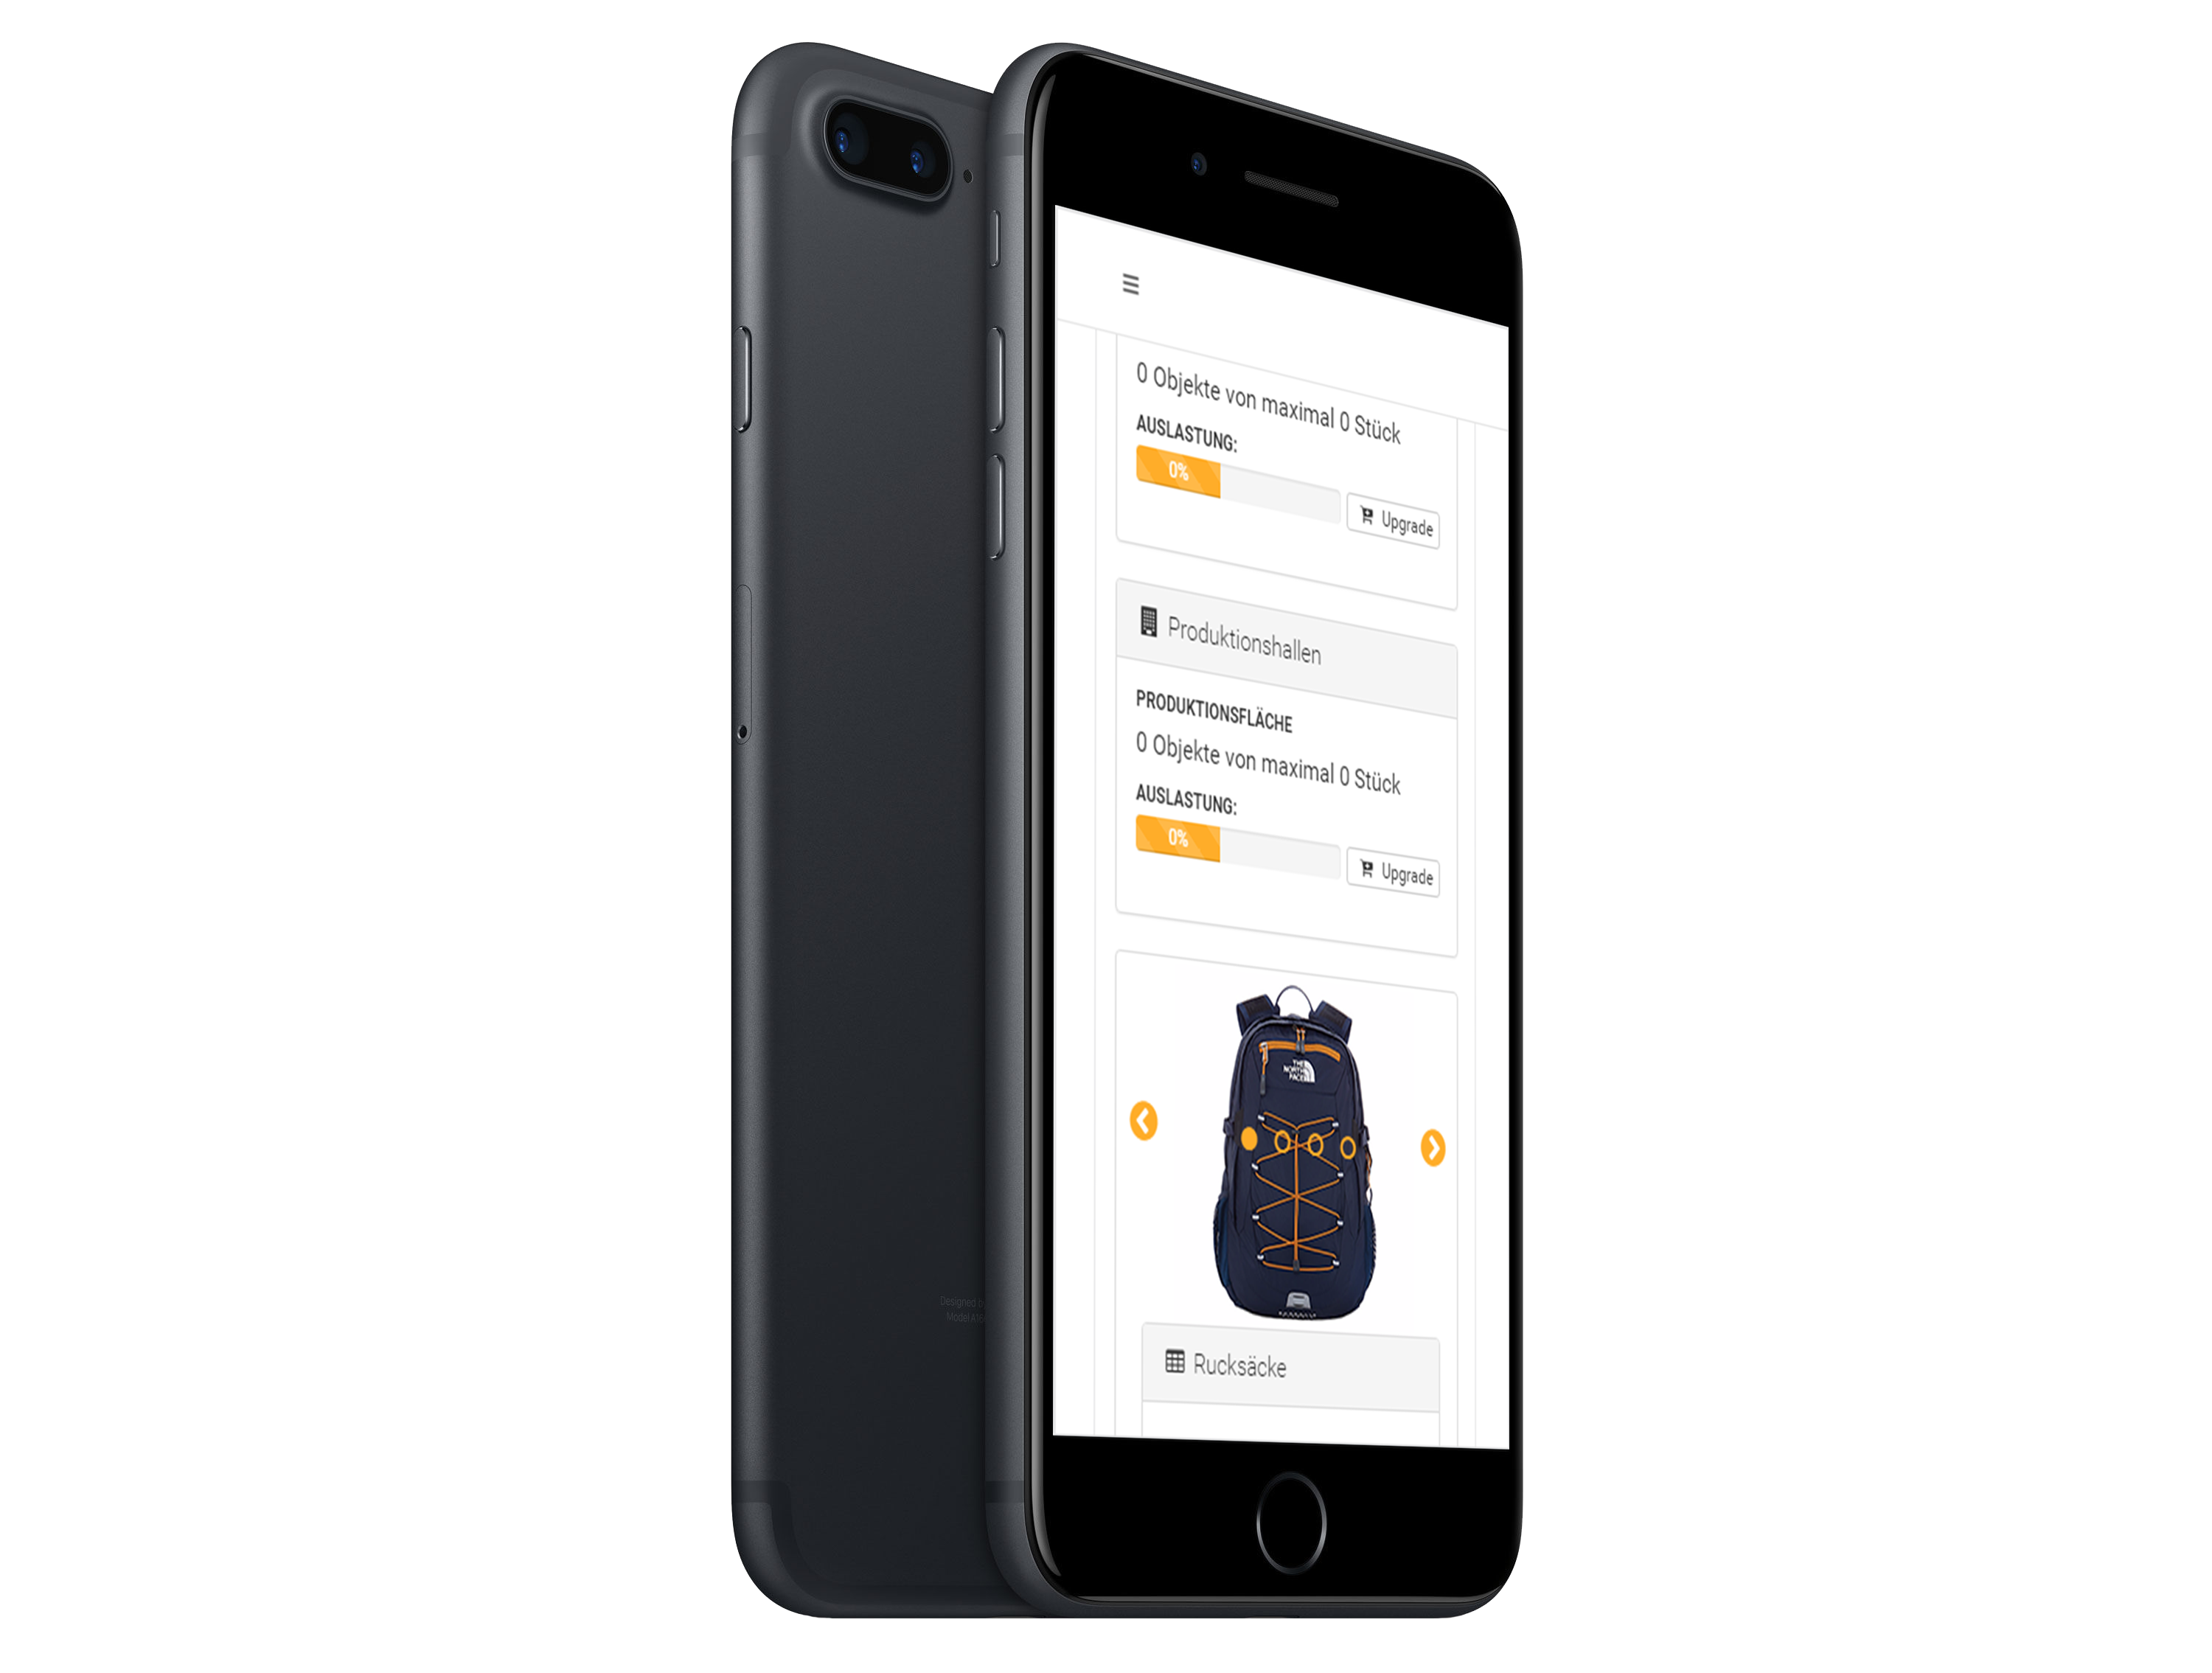
\includegraphics[scale=0.15]{img/mock2.png}
	\captionsetup{format=hang}
	\caption[Seite Produktion Mobile Mockup]{\label{fig:produktion}Seite Produktion Mobile Mockup}
\end{figure}

\subsubsection{Sales \& Accounts}
Die Seite für den Sales liefert die Möglichkeit sich auf Ausschreibungen zu bewerben und somit Deals für sein Unternehmen zu gewinnen. Dabei ist die Seite in zwei identische Spalten aufgeteilt mit jeweils einem \textit{Accordion}. In der linken Spalte sind alle Ausschreibungen als \textit{panel-collapse} Einträge gelistet werden, mit entsprechendem Vertragsschlussdatum und in der rechten Spalte alle aktiven Bewerbungen. Hier werden zusätzlich alle Bewerber auf eine Ausschreibung angezeigt, sowie die Dauer bis Ablauf der Bewerbungsfrist.
\par Die Seite Accounts besteht zum größtenteils aus einer Liste in der alle aktiven Kunden bzw. Deals eingetragen werden. Des weiteren gibt es ein kleines \textit{Panel} in dem die Anzahl der laufenden Verträge, die zu produzierende Menge an Produkten pro Monat und der Momentane Lagerbestand dargestellt wird.

\subsubsection{Research}
Die Reasearch Seite wird genutzt um Forschungen für seine Produktlinien zu starten bzw. in Verbesserungen zu investieren. Neben einem Button für das \textit{Modal} der Seite zum Starten von Forschungen, sind auf der Seite jeweils ein \textit{panel}, welches die aktiven Forschungen anzeigt, sowie alle abgeschlossenen Forschungen. Alle Einträge in den Jeweiligen \textit{panels} erfolgt als \textit{list-group-item} in einer \textit{list-group}.

\subsubsection{Finances}
Die Finances Seite dient als Kostenübersicht für den Spieler. Außerdem können Kredite aufgenommen werden. Die \textit{card} auf der Seite ist gegliedert mit \textit{tabs} welche jeweils pro Jahr hinzugefügt werden, sodass der Spieler jeweils die Kosten und Erlöse für ein Geschäftsjahr anschauen kann. Pro \textit{tab} ist die Seite in zwei Spalten geteilt. Auf der linken Seite sind ein Bilanzstand zum aktuellen Datum abgebildet und die momentane Gewinn- und Verlustrechnung. Beides sind als \textit{table} in einem \textit{panel} eingebunden. Die rechte Spalte ist um einiges kleiner und beinhaltet eine Auflistung von allen laufenden Krediten.

\subsubsection{Anmerkungen zum Frontenddesign}
Ergänzend noch einige Anmerkungen zum Frontenddesign:

\begin{itemize}
\item Aufgrund der Längenbegrenzung der Arbeit wurde nur auf Grobe Elemente in der Seitenbeschreibung eingegangen, nicht auf die genaue implementierung. Diese kann dierekt dem Code entnommen werden.
\item Neben den beschriebenen Seiten gehören noch zusätzliche Elemente zum Design des Frontends, wie z.B. Ladebildschirme, ein Overlay falls das Unternehmen pleite geht oder diverse Fehlermeldungen
\item Neben Bootstrap werden auch einige Semantic UI Elemente verwendet.
\end{itemize}
